\chapter{Evaluation}

In chapter three the requirements for Sparked have been defined via a couple of functional requirements that lead to four workflows:
\begin{itemize}
\item Create an Order
\item Start an Order
\item List existing Orders
\item Display the evaluation data of a completed Order
\end{itemize}

In the same chapter, a handful of guidelines had been developed after which to design the UI.
\begin{itemize}
\item Reduce the information density
\item High contrast, big font
\item Use a strong color to guide the attention 
\item Use the same look and feel throughout the application
\end{itemize}

While creating Sparked, all four of these workflows found their spot in the application. 
 
\begin{figure}
	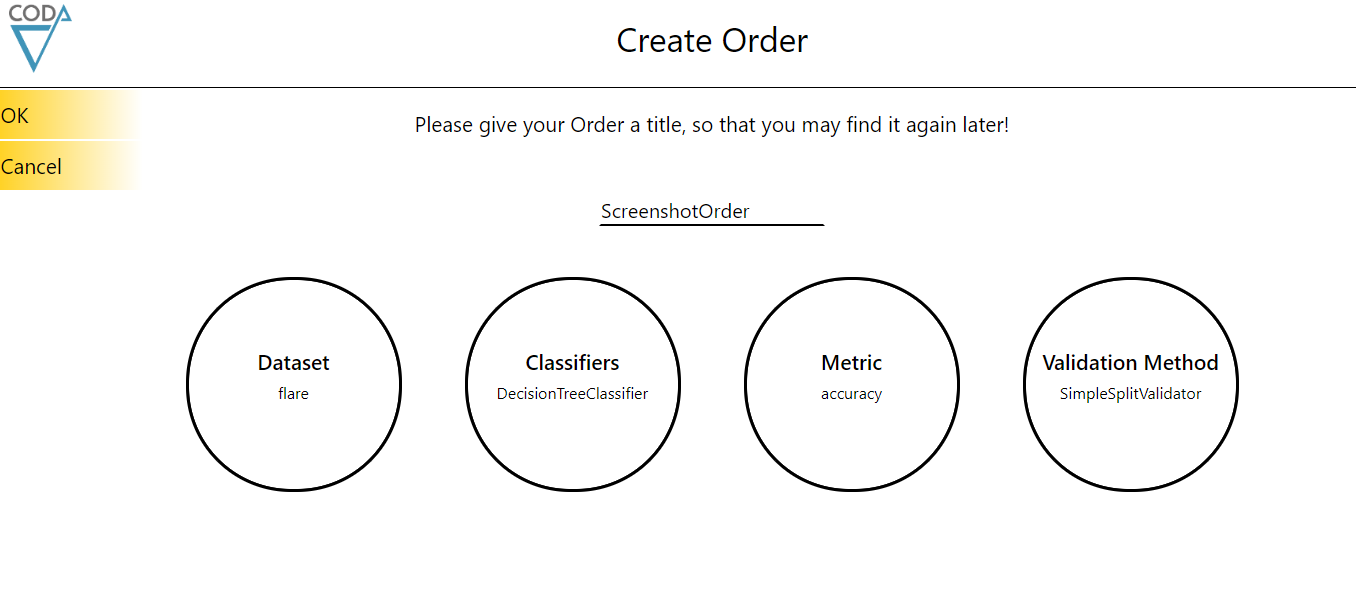
\includegraphics[width=\textwidth]{CreateAnOrder.png}
	\caption{An example of the Create Order workflow.}
\end{figure}

\begin{figure}
	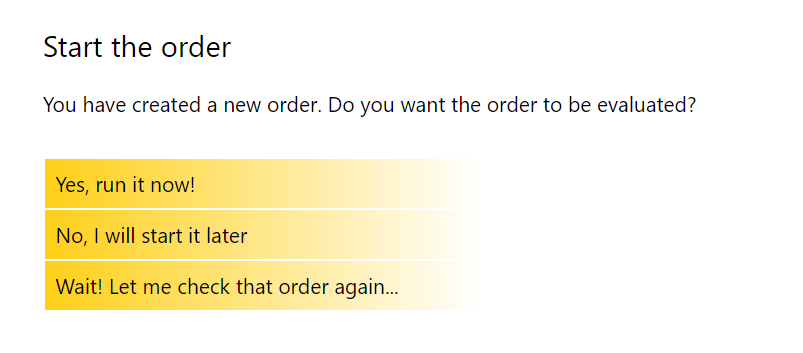
\includegraphics[width=\textwidth]{StartTheOrder.png}
	\caption{Sparked asking for confirmation when finishing an Order.}
\end{figure}

Configuring and starting an Order works. After sending an Order to CODA for evaluation, the listAllEvaluationStatus endpoint shows the Orders combined with a status courtesy of the CODA backend.

\begin{figure}
	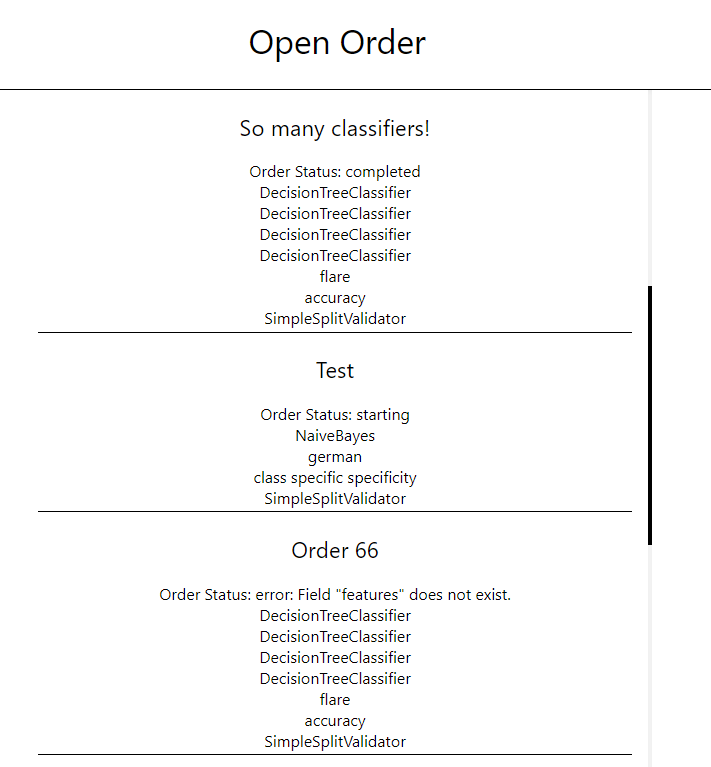
\includegraphics[width=\textwidth]{OrderList.png}
	\caption{List of Orders. The Order Status is supplied by CODA, showing that a connection exists.}
\end{figure}

Opening an Order shows its evaluation page. If the status is completed, the result data is loaded from CODA and displayed together with the general information. The evaluation results are displayed in a bar chart. At the moment this will only display the measurement of the defined evaluation metric. 

\begin{figure}
	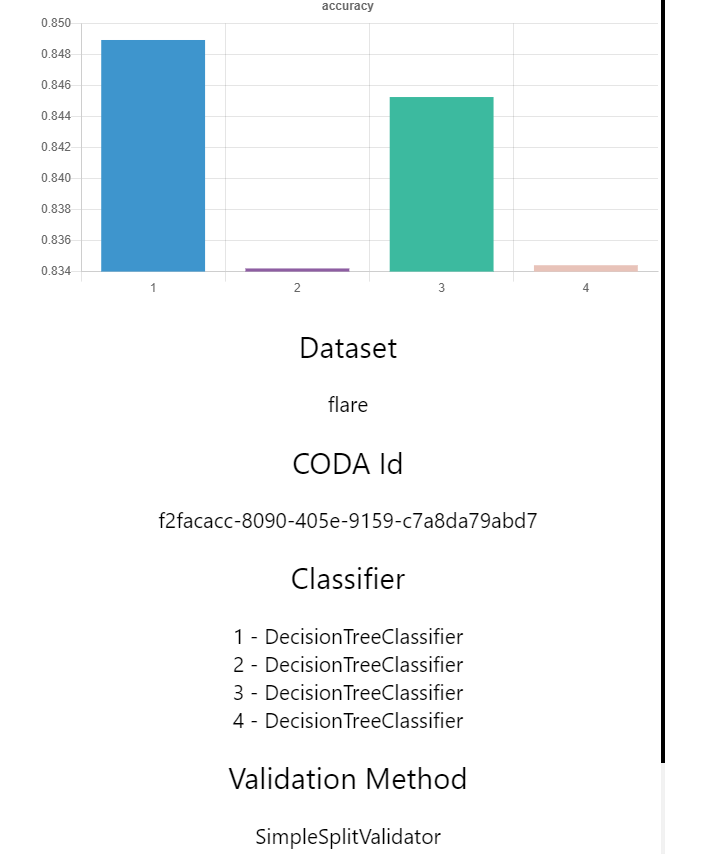
\includegraphics[width=\textwidth]{ShowEvaluationMetric.png}
	\caption{An Order created via Sparked with visualized result data. All workflows have to work to get to this point.}
\end{figure}

Next to others an Order with the flare dataset, four decision tree classifiers with different hyperparameters, accuracy as evaluation method and a simple split validator was created and subsequentially started. The order was successfully evaluated and the data shown on the evaluation page (IMAGE X+Z), showing that all parts work in tandem. 

In an attempt to test readability of the Sparked UI under bad lighting conditions the UI was projected onto a screen while having strong if indirect sunlight (Image X+Y). As expected, the UI looks washed out but is still easily readable.

\begin{figure}
	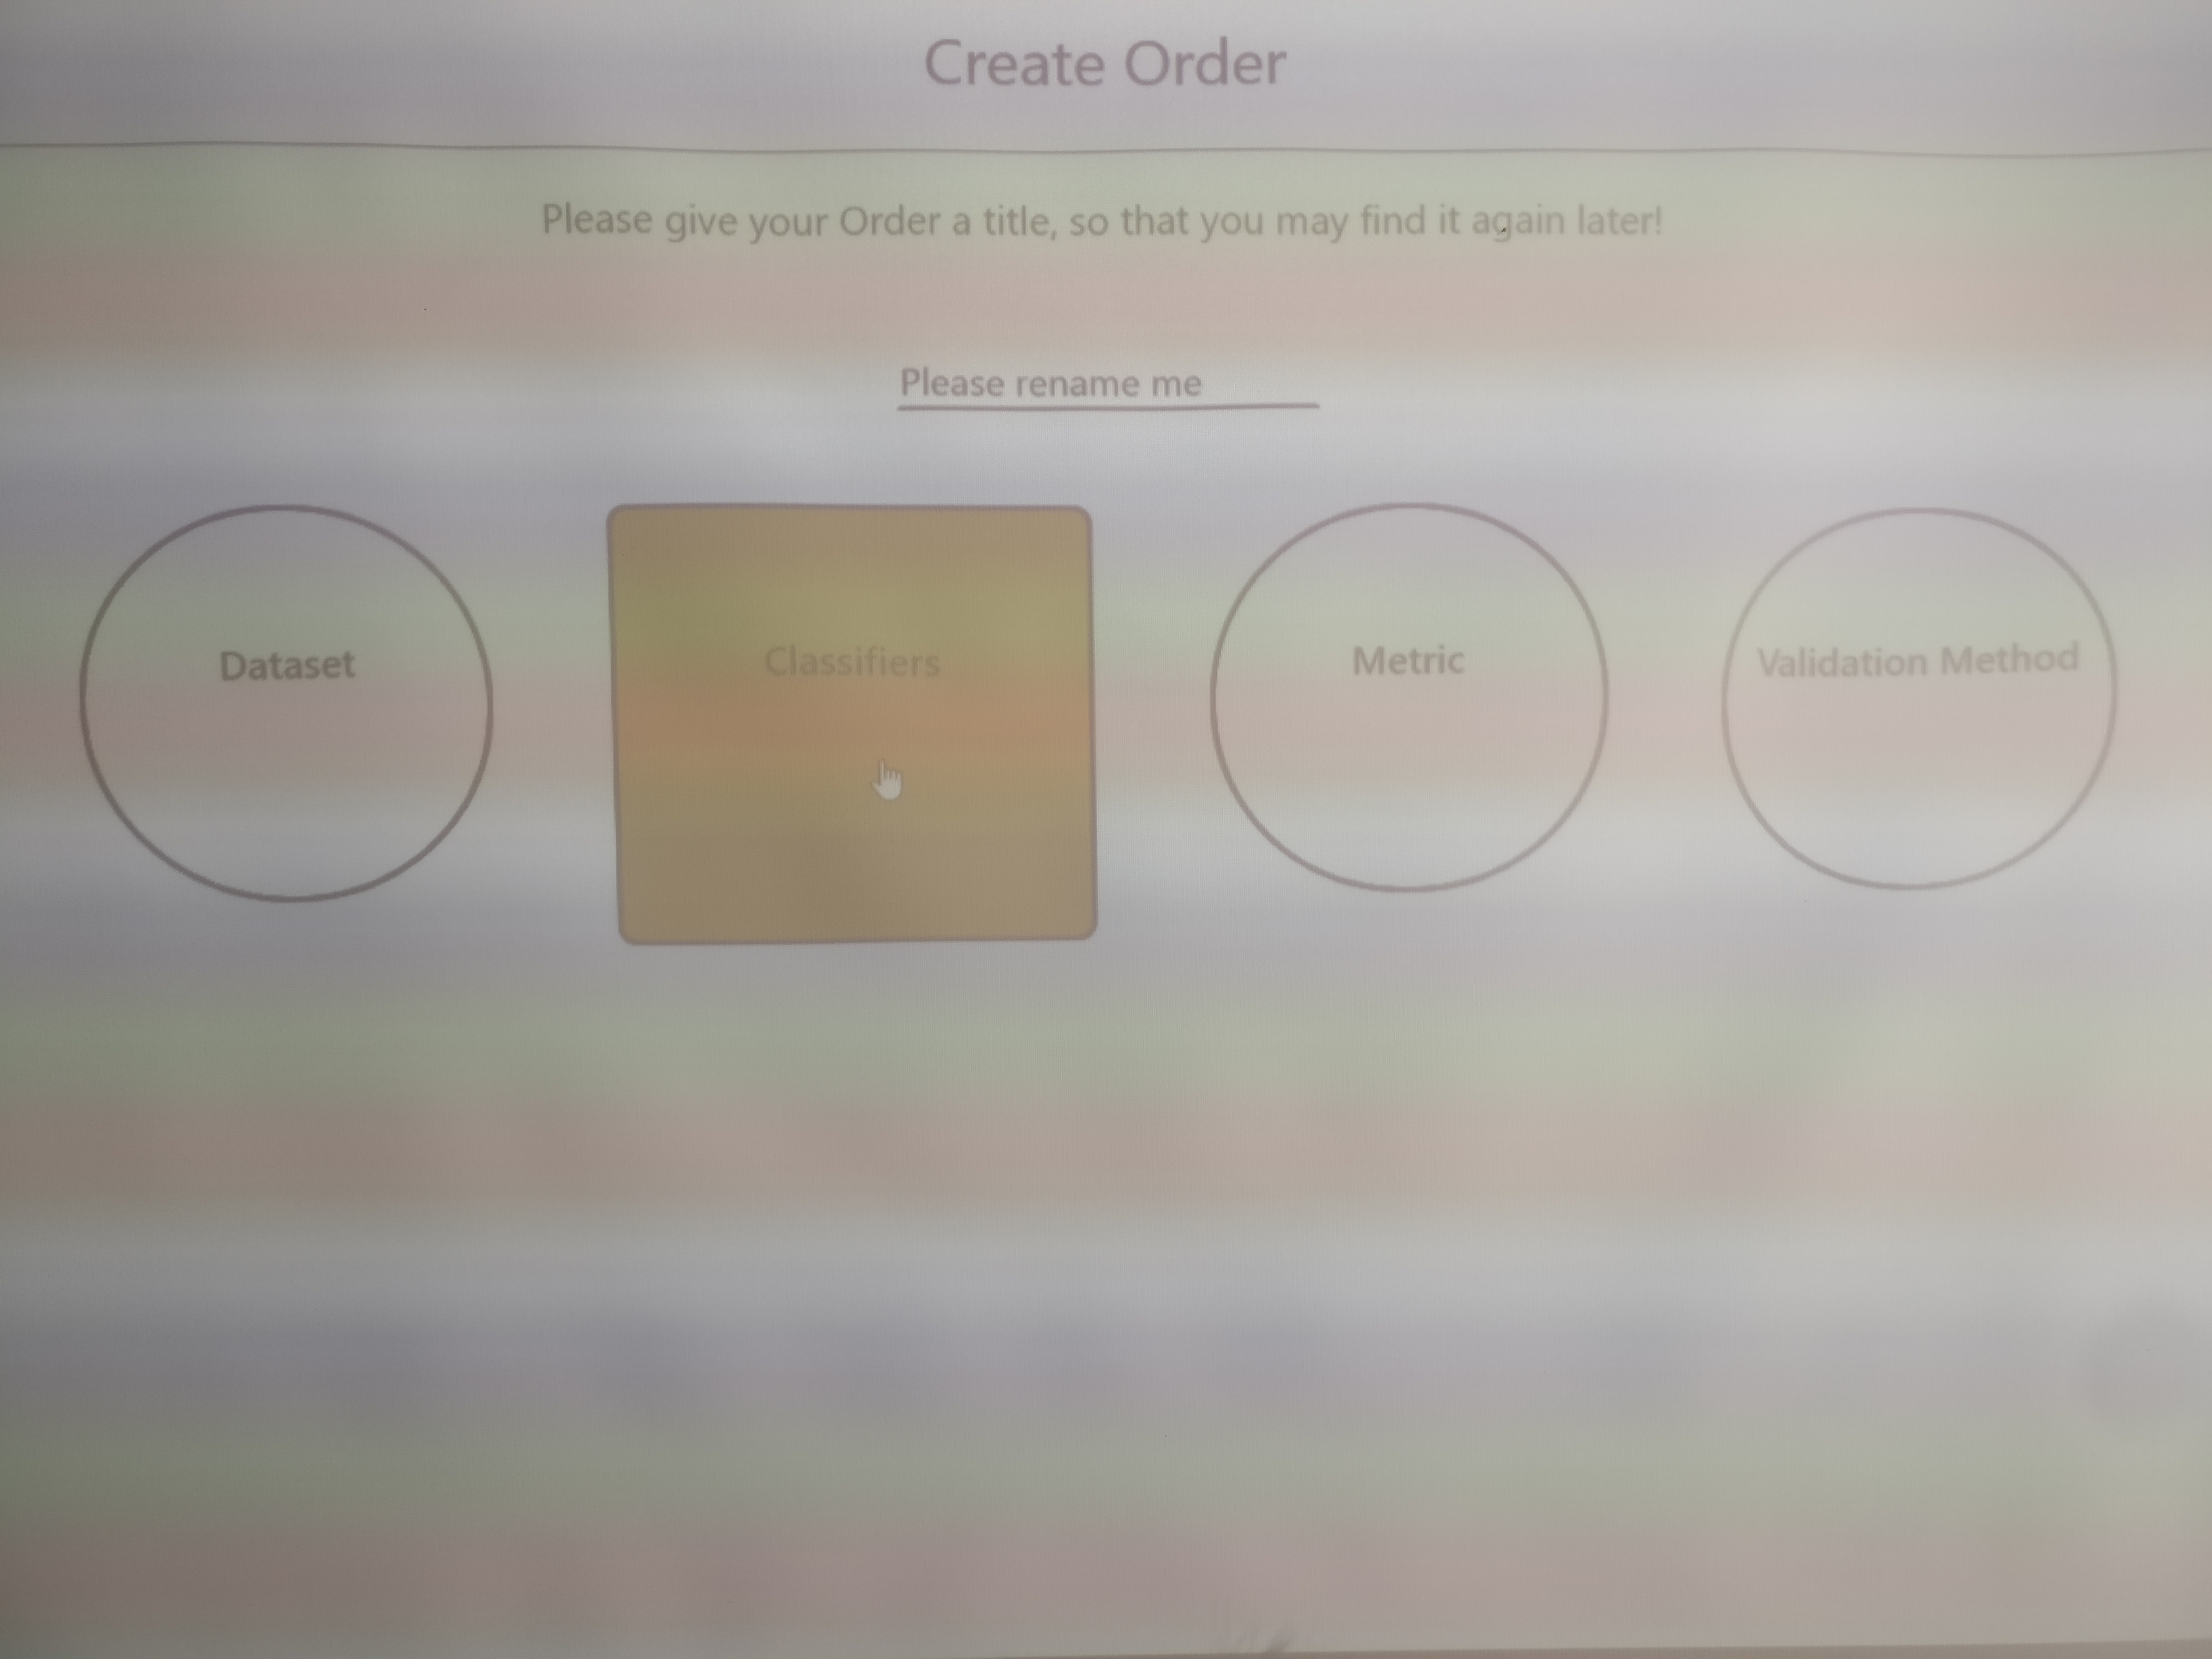
\includegraphics[width=\textwidth]{SparkedBadLighting.jpg}
	\caption{The Sparked UI on a beamer in a bright room with indirect but strong sunlight photographed with a smartphone camera.}
\end{figure}
